\section{Theorie}
\subsection{Bindungstypen in Kristallen}
\subsubsection{Van-der-Waals-Wechselwirkung}
Diese Kraft ist relativ schwach und wird erst bei vielen Atomen relevant. Sie entsteht durch ein gegenseitig induziertes Dipolmoment als Wirkung von Fluktuationen in der Ladungsverteilung der Atome. Das rührt daher, dass die Ladungsverteilung nicht starr ist.

\noindent Die Kraft fällt mit der negativ reziproken sechsten Potenz des Abstandes und ist somit sensitiv gegenüber Schwankungen.

\noindent Da es bei der STM zwei Modi gibt, einmal die Variation des Abstandes und das konstant Halten des Tunnelstroms und einmal die Variation des Stromes und das konstant Halten des Abstandes, wobei erstes als Rasterkraftmikroskopie gilt, ist die Van-der-Waals-Kraft auch nur für diese wichtig.

\subsubsection{Repulsive Wechselwirkung}
Wird die Spitze bei der Rasterkraftmikroskpie zu nah an die Probe gefahren, tritt eine abstoßende Kraft zwischen Spitze und Probe ein. Diese wird repulsive Wechselwirkung genannt. Sie entsteht durch das Überlappen der Elektronenladungsverteilungen unter Berücksichtigung des Paulischen Ausschließungsprinzips.

\noindent Ein empirisch abgeleitetes Potential, welches die Herkunft dieser Kraft beschreibt, ist das Lennard-Jones-Potential.

\begin{equation}
U_\text{LJ}(R)=4\epsilon\left[\frac{\sigma}{R}^12-\frac{\sigma}{R}^6\right]
\end{equation}

\subsection{Tunneleffekt}
Die Funktionsweise des Rastertunnelmikroskops basiert auf dem quantenmechanischen Phänomen des Tunneleffekts. Ist ein Wellenpaket von einer endlich hohen Potentialbarriere eingeschlossen, kann es diese im klassischen Fall nicht durchdringen. Quantenmechanisch ist dies jedoch möglich, da das Wellepaket durch eine Lösung der Schrödingergleichung beschrieben werden kann, die im Betragsquadrat lediglich Information über die Aufenthaltswahrscheinlichkeit des Wellenpakets liefert. Diese Wahrscheinlichkeit ist außerhalb der Potentialbarriere ungleich null, sodass das Wellenpaket durchaus hinter der Barriere auffindbar sein kann. 

\noindent Bei der STM wird ein elektrisch leitender oder mit einem solchen Material überzogener Festkörper untersucht, indem eine Pt-Ir-Drahtspitze an eine Probe genähert wird, die dann über diese rastert. Es existiert also ein Valenzband in dem sich Elektronen der Fermienergie befinden. Die zu überwindende Potentialbarriere für den Tunneleffekt in diesem Versuch ist das Vakuum. Der Effekt ist nur für Abstände in atomischer Skala relevant, weswegen eine typische Probe der Größenordnung 100\,\r{A}\(^2\) ist und der Versuchsaufbau dementsprechend sensitiv gegenüber dem Abstand zwischen Spitze und Probe ist. Eine Genauigkeit von 1\,\r{A} für die Spitze kann beim Anlegen einer Spannung von \(0,1\)V erreicht werden.

\noindent Wird eine Spitze in die Nähe einer Probe mit diesen Eigenschaften gebracht, kann der Tunneleffekt für die Elektronen der Spitze oder für die der Probe eintreten, was davon abhänging ist, welches Vorzeichen die an die Spitze angelegte Spannung hat. Es entsteht ein Tunnelstrom, der gemessen werden kann.

\noindent Der Tunnelstrom fällt exponentiell mit dem Abstand \(d\) und der Wurzel der Austrittsarbeit \(\Phi\) des Festkörpers. Dies ist die Energie, die mindestens aufgewandt werden muss, um ein Elektron aus einem ungeladenen Festkörper zu lösen. 

\begin{equation}
I_\text{T}=\frac{U}{d}\exp{(-Kd\sqrt{\Phi})},\quad K\approx1,025\frac{1}{\text{\r{A}}\,\text{eV}^\frac12}
\end{equation}

\noindent Daraus ergeben sich direkt die zwei Hauptschwierigkeiten dieses Versuchs. Zum einen muss der gesamte Versuchsaufbau bezüglich mechanischer Vibrationen in der Größenordnung von \(<1\)\,\r{A} gedämpft werden, da der Abstand \(d\approx0,5\)\,\r{A} anfällig auf sehr schwache Schwingungen ist.  

\noindent Zum anderen muss die Drahtspitze möglichst spitz und sauber präpariert sein. Das heißt der Draht wird vor der Benutzung mit 2-Propanol von lipophilem Dreck befreit.

\subsection{Fehlerquellen}
\subsubsection{Intrinsische Nichtlinearität}
Dieser Fehler ergibt sich aus der Längenänderung des Scanners (piezoelektrischer Stab) nach dem Anlegen einer Spannung. Da die Spannung nicht instantan angelegt wird, sondern sich über Zeit aufbaut ist die Längenänderung des Stabes als Funktion der Spannung keine lineare Gerade.

\begin{figure}
	\centering
		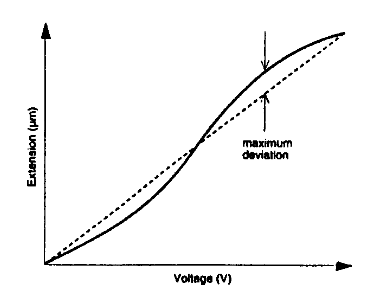
\includegraphics[width=0.5\textwidth]{nichtlinearitat.png}
	\caption{Längenänderung über Spannung}
	\label{fig:nichtlinearität}
\end{figure}

\noindent Die intrinsische Nichtlinearität ist also ein Maß für die maximale Auslenkung des Stabes im Verhältnis zu der Auslenkung des Stabes bei fester Spannung. 

\noindent Dieser Effekt spiegelt sich bei der Abtastung wieder, indem das abgefahrene Muster eine gewisse Verzerrung aufweist, statt einem Rasterschema wie in Abbildung \ref{fig:raster}.

\begin{figure}
	\centering
		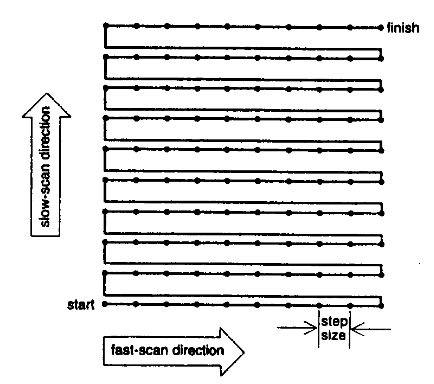
\includegraphics[width=0.5\textwidth]{raster.png}
	\caption{Raster des Scanners}
	\label{fig:raster}
\end{figure}

\noindent Die Reichweite einer typischen Nichtlinearität erstreckt sich von 2\% bis 25\%.

\subsubsection{Hysterese}
Bei der Ausdehnung eines Piezokristalls unter Anlegen einer Spannung tritt Hysterese auf.
Das bedeutet für die Messung, dass bei einer Bewegung der Spitze in positiver X-Richtung andere Werte gemessen werden als in negativer X-Richtung.

Um dennoch sinnvolle Ergebnisse zu erhalten, werden alle Messwerte bei gleicher Bewegungsrichtung aufgenommen.

\subsubsection{Kriechen}
Die Reatkion des Piezokristalls auf eine Spannungsänderung findet im Idealfall instantan statt.
In der Realität lässt sich die Bewegung in zwei Teile aufteilen.
Der erste Teil der Bewegung findet in weniger als einer Millisekunde statt, während der zweite Teil länger dauert.
Der Kriechfaktor gibt das Verhältnis der Strecken vom ersten und zweiten Teil an.

Eine Folge dieses Effekts ist, dass Messungen, die mit unterschiedlicher Geschwindigkeit durchgeführt werden, unterschiedliche Ergebnisse liefern.

\subsubsection{Alterung}
Die Ausrichtung der Dipole im Piezokristall wird durch Anlegen von Spannung beeinflusst.
Ebenso hebt sich die Ausrichtung der Dipole bei längerer Lagerung auf.
Als Folge davon ändert sich der Belastungskoeffizient des Piezokristalls und die Position auf der X, Y und Z-Achse wird verfälscht.

\subsubsection{Kreuzkopplung}

Die Aufhängung der Spitze besteht aus drei Piezo-Röhren, die am Ende verbunden sind.
Das Strecken oder Stauchen einer Röhre führt deshalb nicht, wie gewünscht, zu einer Translationsbewegung auf einer Achse, sondern zu einer Art Schwenkbewegung auf mehreren Achsen.
Die ungewünschte Bewegung entlang der anderen Achsen wird als Kreuzkopplung bezeichnet.

Die Kreuzkopplung wird entweder durch Software korrigiert oder die Spitze wird durch eine Regelschleife an die korrekte Stelle gefahren.

\subsubsection{Thermische Effekte}
Erwärmung und Abkühlung der Messspitze bzw. der Probe können den Tunnelstrom verändern und somit die Messung verfälschen.
Deshalb sollten die Spitze und Probe nicht berührt werden.
Außerdem wird ein Glasgefäß über das Mikroskop gestülpt, um Luftaustausch zu vermeiden.